\documentclass{article} 
\usepackage{tikz}
\usepackage{pgfplots}
\usepackage{geometry}
\usepackage{amsmath}
\usepackage{amssymb}
\geometry{margin=1in}
\pgfplotsset{every tick label/.append style={font=\small}}
\title{CS3244 Machine Learning
\\ Homework 2 (Essay Questions) } 
\author{Matric No. - A0153196B}
\begin{document} 

\maketitle{} 
\section*{2.}
\textbf{Consider the following training data:}
\begin{center}
\begin{tabular}{ ||c | c | c || } 
 \hline
$x_1$ & $x_2$ & y \\ [0.5 ex] 
\hline
\hline
 1 & 1 & + \\ 
 \hline
 2 & 2 & + \\ 
 \hline
 2 & 0 & + \\
 \hline
 0 & 1 & - \\
 \hline
 1 & 0 & - \\ 
\hline
 0 & 0 & - \\
 \hline
\end{tabular}
\end{center}
\textbf{a. Plot these six training points. Are the classes $\left\lbrace +, − \right\rbrace$ linearly separable?} 
\\~\\
 \underline{ANS.} Yes these classes are linearly separable. The plot is shown below :-
\\~\\
\begin{tikzpicture}
\begin{axis}[
  axis x line=center,
  axis y line=center,
  xtick={-1,0,...,3},
  ytick={-1,0,...,3},
  xlabel={$x_1$},
  ylabel={$y_1$},
  xlabel style={above right},
  ylabel style={above right},
  label style={font=\Large},
  xmajorgrids = true,
  ymajorgrids = true,
  xmin=-1,
  xmax=3,
  ymin=-1,
  grid style=dashed,
  ymax=3]
  \addplot[only marks, mark = *,mark options={fill=blue},color = blue] coordinates {
 	(1,1)
 	(2,2)
 	(2,0)
 };
 \addplot[only marks, mark = *,mark options={fill=red},color = red] coordinates {
 	(0,1)
 	(1,0)
 	(0,0)
 };
 \end{axis}
 \end{tikzpicture}
 \\~\\
\textbf {b. Construct the weight vector of the maximum margin hyper-plane by inspection and identify the support vectors.}
\\~\\
\underline{ANS.} The margin and hyperplane are given below :-
\\~\\
 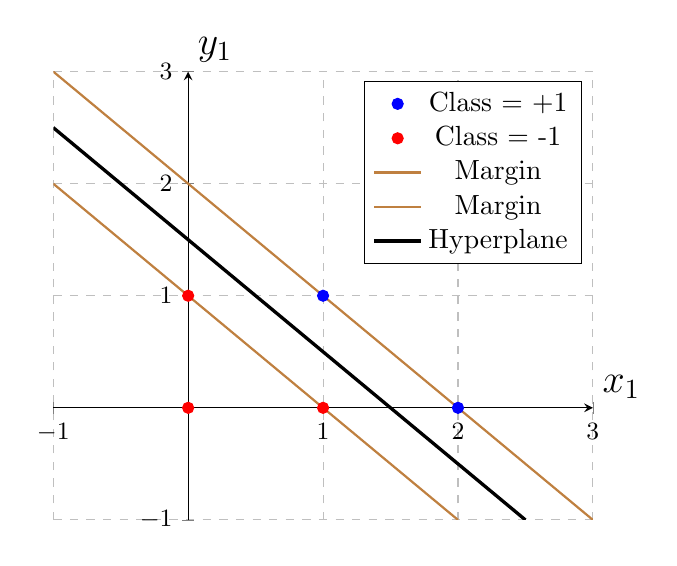
\begin{tikzpicture}
 \begin{axis}[
  axis x line=center,
  axis y line=center,
  xtick={-1,0,...,3},
  ytick={-1,0,...,3},
  xlabel={$x_1$},
  ylabel={$y_1$},
  xlabel style={above right},
  ylabel style={above right},
  label style={font=\Large},
  xmajorgrids = true,
  ymajorgrids = true,
  xmin=-1,
  xmax=3,
  ymin=-1,
  grid style=dashed,
  ymax=3]
  \addplot[only marks, mark = *,mark options={fill=blue},color = blue] coordinates {
 	(1,1)
 	(2,2)
 	(2,0)
 };
 \addlegendentry { Class = +1 }
 \addplot[only marks, mark = *,mark options={fill=red},color = red] coordinates {
 	(0,1)
 	(1,0)
 	(0,0)
 };
 \addlegendentry { Class = -1 }
 \addplot[no marks, mark = *,color = brown,thick] coordinates {
 	(0,1)
 	(1,0)
 	(-1,2)
 	(2,-1)
 };
 \addlegendentry { Margin }
 \addplot[no marks, mark = *,color = brown,thick] coordinates {
 	(-1,3)
 	(2,0)
 	(1,1)
 	(3,-1)
 };
 \addlegendentry { Margin }
 \addplot[no marks, mark = *,color = black,very thick] coordinates {
 	(-1,2.5)
 	(1,1/2)
 	(1/2,1)
 	(2.5,-1)
 };
 \addlegendentry { Hyperplane }
 \end{axis}
\end{tikzpicture}
\\
The equations of the margin, hyperplane, weight vector and support vectors are as follows:- 
\begin{center}
\textbf{Margin (Class +1): } $x_1 + x_2 - 2 = 0$ \\
\textbf{Margin (Class -1): } $x_1 + x_2 - 1 = 0$ \\
\textbf{Hyperplane: } $x_1 + x_2 - 1.5 = 0$
\[
\textbf{Normalized weight vector: } 
	\frac{1}{\sqrt{2}}
	\begin{bmatrix} 
	1 \\
	1  
	\end{bmatrix}
\]
\[
\textbf{Support Vectors: } 
	\begin{bmatrix} 
	2 \\
	0  
	\end{bmatrix}
	\begin{bmatrix} 
	1 \\
	1  
	\end{bmatrix}
	\begin{bmatrix} 
	1 \\
	0  
	\end{bmatrix}
	\begin{bmatrix} 
	0 \\
	1  
	\end{bmatrix}	
\]
\end{center}
\textbf {c. If you remove one of the support vectors, does the size of the optimal margin decrease, stay the same, or increase? Explain.}
\\~\\
\underline{ANS.} If we remove one of the support the margin will still \textbf{stay the same} because no matter which support vector we remove, the optimal margin is still passing through other three support vectors which will keep it intact. Since a support vector is the nearest point to the hyperplane, removing it means that we have to consider the next nearest point in our dataset which can only increase the margin or keep it fixed depending on the presence of other support vectors. A supporting figure is shown below:-
\begin{center}
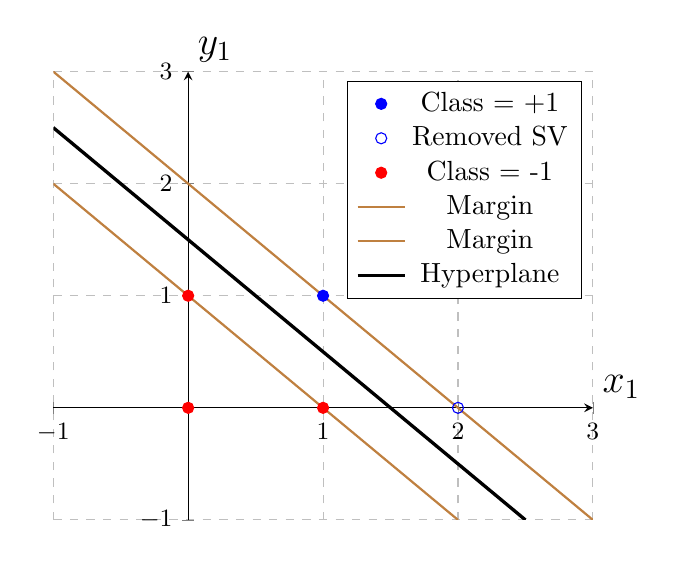
\begin{tikzpicture}
 \begin{axis}[
  axis x line=center,
  axis y line=center,
  xtick={-1,0,...,3},
  ytick={-1,0,...,3},
  xlabel={$x_1$},
  ylabel={$y_1$},
  xlabel style={above right},
  ylabel style={above right},
  label style={font=\Large},
  xmajorgrids = true,
  ymajorgrids = true,
  xmin=-1,
  xmax=3,
  ymin=-1,
  grid style=dashed,
  ymax=3]
  \addplot[only marks, mark = *,mark options={fill=blue},color = blue] coordinates {
 	(1,1)
 	(2,2)
 };
 \addlegendentry { Class = +1 }
 \addplot[only marks, mark = o,mark options={fill=blue},color = blue] coordinates {
 	 (2,0)
 };
 \addlegendentry {Removed SV}
 \addplot[only marks, mark = *,mark options={fill=red},color = red] coordinates {
 	(0,1)
 	(1,0)
 	(0,0)
 };
 \addlegendentry { Class = -1 }
 \addplot[no marks, mark = *,color = brown,thick] coordinates {
 	(0,1)
 	(1,0)
 	(-1,2)
 	(2,-1)
 };
 \addlegendentry { Margin }
 \addplot[no marks, mark = *,color = brown,thick] coordinates {
 	(-1,3)
 	(2,0)
 	(1,1)
 	(3,-1)
 };
 \addlegendentry { Margin }
 \addplot[no marks, mark = *,color = black,very thick] coordinates {
 	(-1,2.5)
 	(1,1/2)
 	(1/2,1)
 	(2.5,-1)
 };
 \addlegendentry { Hyperplane }
 \end{axis}
\end{tikzpicture}
\end{center}
We can see in the above figure that the support vector at (2,0) has been removed but the margin stays the same because of the presence of the vector at (1,1).
\\~\\
\textbf{d. Is your answer to (c) also true for any dataset? Provide a counterexample or give a short proof.}
\\~\\
\underline{ANS.} The answer to (c) is not true for every dataset. There can be cases when the margin increases. However, it will never decrease in case of a hard margin svm. We can show this with the help of a counterexample. Consider a dataset which consists of 3 points shown below:-
\begin{center}
\begin{tabular}{ ||c | c | c || } 
 \hline
$x_1$ & $x_2$ & y \\ [0.5 ex] 
\hline
\hline
 1 & 0 & - \\ 
 \hline
 1 & 1 & + \\ 
 \hline
 2 & 2 & + \\
 \hline
\end{tabular}
\end{center}
\[
{The plot of this data is given below. It has 2 support vectors }
\begin{bmatrix} 
	1 \\
	0  
	\end{bmatrix}
	\begin{bmatrix} 
	1 \\
	1  
	\end{bmatrix}
{Now if we remove the support vector }
	\begin{bmatrix} 
	1 \\
	1  
	\end{bmatrix}
we will get the figure shown on the right hand side.
\]
\section*{3.}
\textbf{A kernel is valid if it corresponds to a scalar product in some (perhaps infinite dimensional) feature space. Remember a necessary and sufficient condition for a function K(x, x) to be a valid kernel is that associated Gram matrix, whose elements are given by k(xn,xm), should be positive semi-definite for all possible choices of the set x. Show whether the following are also kernels:}
\\~\\
Valid kernels follow the following properties which we are going to use in our proof:- 
\\~\\
\begin{center}
\textit{\underline{Property 1:} Given two valid kernels $K_1$(-,-) and $K_2$(-,-):} \\
K(\textbf{x},\textbf{x$'$}) = $K_1$(\textbf{x},\textbf{x$'$}) + $K_2$(\textbf{x},\textbf{x$'$})
\\~\\
\textit{\underline{Property 2:} Given two valid kernels $K_1$(-,-) and $K_2$(-,-):} \\
K(\textbf{x},\textbf{x$'$}) = $K_1$(\textbf{x},\textbf{x$'$}) * $K_2$(\textbf{x},\textbf{x$'$}) 
\\~\\
\textit{\underline{Property 3:} Given a valid kernel $K_1$(-,-):} \\
K(\textbf{x},\textbf{x$'$}) = q[$K_1$(\textbf{x},\textbf{x$'$})]\\
\textit{where q[.] is a polynomial function with non-negative coefficients.}

\end{center}
1. K(\textbf{x},\textbf{x$'$}) = c$\langle \textbf{x},\textbf{x$'$} \rangle$
\\~\\
\underline{ANS.} \\
First of all, $\langle \textbf{x},\textbf{x$'$} \rangle$ is a valid kernel since it represents a scalar product in the Euclidean space. Inner products are \textbf{symmetric} and their Gram Matrices are \textbf{positive semi-definite} which are the essential conditions of being a valid kernel. 
\\~\\
Assuming c is non negative i.e. c $>$ 0 we can use \textit{Property 3} here as c$\langle \textbf{x},\textbf{x$'$} \rangle$ is a polynomial function of $\langle \textbf{x},\textbf{x$'$} \rangle$ with degree 1 and non negative coefficients (c).
\begin{center}
 Let $K_1$(\textbf{x},\textbf{x$'$}) = $\langle \textbf{x},\textbf{x$'$} \rangle$ 
 \\~\\
$\therefore$    q[ $K_1$(\textbf{x},\textbf{x$'$}) ] = q[ $\langle \textbf{x},\textbf{x$'$} \rangle$ ] = c$\langle \textbf{x},\textbf{x$'$} \rangle$ \quad where c $>$ 0
\end{center}

Since $\langle \textbf{x},\textbf{x$'$} \rangle$ is a valid kernel, q[ $\langle \textbf{x},\textbf{x$'$} \rangle$ ] is also a valid kernel. \\
$\therefore$ \quad c$\langle \textbf{x},\textbf{x$'$} \rangle$ is a valid kernel. 

\\~\\~\\

2. K(\textbf{x},\textbf{x$'$}) = $\langle \textbf{x},\textbf{x$'$} \rangle^2$ + $e^{(-||x||^2)}$$e^{(-||x'||^2)}$
\\~\\
\underline{ANS.} \\
Again as a base case $\langle \textbf{x},\textbf{x$'$} \rangle$ is a valid kernel due to reasons specified in the previous question. We will prove that the given kernel function is valid by first showing that the individual components are valid:-
\\~\\
\underline{Proof for $\langle \textbf{x},\textbf{x$'$} \rangle^2$ :} \\
\begin{center}
Let \quad $K_1$(\textbf{x},\textbf{x$'$}) = $K_2$(\textbf{x},\textbf{x$'$}) = $\langle \textbf{x},\textbf{x$'$} \rangle$ 
\end{center}
Since $\langle \textbf{x},\textbf{x$'$} \rangle$ is valid $K_1$(\textbf{x},\textbf{x$'$}) and $K_2$(\textbf{x},\textbf{x$'$}) are also valid. 
\begin{center}
K(\textbf{x},\textbf{x$'$}) = $K_1$(\textbf{x},\textbf{x$'$}) * $K_2$(\textbf{x},\textbf{x$'$}) = $\langle \textbf{x},\textbf{x$'$} \rangle^2$
\end{center}
Using \textbf{\textit{Property 2}}, since $K_1$(\textbf{x},\textbf{x$'$}) and $K_2$(\textbf{x},\textbf{x$'$}) are valid K(\textbf{x},\textbf{x$'$}) is also valid \\
\begin{center}
$\therefore$ \quad $\langle \textbf{x},\textbf{x$'$} \rangle^2$ is a valid kernel
\end{center}
\\
\underline{Proof for $e^{(-||\textbf{x}||^2)}$$e^{(-||\textbf{x$'$}||^2)}$ :} 
\\~\\
We know that a kernel is valid if it is \textbf{symmetric} and \textbf{positive semidefinite}. Let's prove these properties individually:- \\
\begin{itemize}
\item Symmetry: 
    \begin{center}
    Let K(\textbf{x},\textbf{x$'$}) = $e^{(-||\textbf{x}||^2)}$$e^{(-||\textbf{x$'$}||^2)}$ 
    \\~\\
    K(\textbf{x},\textbf{x$'$}) = $e^{(-||\textbf{x}||^2)}$$e^{(-||\textbf{x$'$}||^2)}$ = $e^{(-||\textbf{x$'$}||^2)}$$e^{(-||\textbf{x}||^2)}$ = K(\textbf{x$'$},\textbf{x})
    \\~\\
    $\therefore$ \quad $e^{(-||\textbf{x}||^2)}$$e^{(-||\textbf{x$'$}||^2)}$ is symmetric.
    \end{center}
\item Positive semi-definiteness:
    \\~\\
    According to \textbf{Mercer's Theorem}: \\
    \textit{A symmetric function K(x, y) can be expressed as an inner product
      \begin{center}
      K(\textbf{x},\textbf{x$'$}) = $\langle \phi(\textbf{x}),\phi(\textbf{x$'$}) \rangle$
      \end{center}
      for some mapping $\phi$ \textbf{if and only if} K(\textbf{x},\textbf{x$'$}) is positive semidefinite 
      }
      \\~\\
      Thus, if we are able to find a mapping $\phi$ for the given function, it means that the function is positive semidefinite according to Mercer's theorem.
      \\~\\
      Consider \quad $\phi(x)$ = $e^{(-||\textbf{x}||^2)}$ \\
      Then \quad K(\textbf{x},\textbf{x$'$}) = $\langle \phi(\textbf{x}),\phi(\textbf{x$'$}) \rangle$ = $\langle $e^{(-||\textbf{x}||^2)}$,$e^{(-||\textbf{x$'$}||^2)}$ \rangle$ = $e^{(-||\textbf{x}||^2)}$$e^{(-||\textbf{x$'$}||^2)}$
    }
\end{itemize}
A symmetric function K(\textbf{x},\textbf{x$'$}) is a kernel is valid if it can be expressed as an inner product in some feature space. In other words:- 
\begin{center}
K(\textbf{x},\textbf{x$'$}) = $\langle \textbf{x},\textbf{x$'$} \rangle$ 
\end{center}
\end{document}